\documentclass[
    a4paper,
    12pt,
    mathserif,
    handout
    ]{beamer}
%\usefonttheme[onlymath]{serif}

\usepackage{FabZ}
\usepackage{vecteurs}

%\usepackage[T1]{fontenc}
%\usepackage[utf8x]{inputenc}
%\usepackage[frenchb]{babel}


\usetheme{default}
\usecolortheme{default}

%\usetheme{Darmstadt}
%\usetheme{Copenhagen}
%\usecolortheme{beaver}

%\usecolortheme{crane}
%\usecolortheme{rose}
%\usecolortheme{seahorse}


\usepackage{graphicx}
\usepackage{hyperref}

%\author{\textsc{Fabien S\'eries}}
\date{~}
\title{Repérage dans le plan}
%\subtitle{NonDestructive Testing}
%\institute{
%%\includegraphics[width=0.2\textwidth]{./../pictures/itwm_85mm_cmyk.eps}
%}

\begin{document}

%% boite en couleur avec titre plus fonce
%\definecolor{fondtitre}{rgb}{0.5,0.5,1}
%\definecolor{coultitre}{rgb}{0.0,0.5,0.5}

% barre de navigation (page précedente, zoom...)
\setbeamertemplate{navigation symbols}{%
% \insertslidenavigationsymbol
% \insertframenavigationsymbol
% \insertsubsectionnavigationsymbol
% \insertsectionnavigationsymbol
% \insertdocnavigationsymbol
% \insertbackfindforwardnavigationsymbol
}

%% Permet lors d'une liste qui doit afficher certains de ses éléments dans le transparent d'après de le mettre en transparent (voir transparent 5)
\beamertemplatetransparentcovered

%\setbeamertemplate{caption}[numbered] %% Pour mettre des numéros aux figures

% Chaque page contiendra en bas à droite la position actuelle sur le nombre de transparents
%\logo{\footnotesize{\insertframenumber/\inserttotalframenumber}}
% Afficher le texte dans \logo{} avec des couleurs et pas en gris qu'on voit pas !!
%\setbeamercolor{logo}{parent=palette primary}

%\setbeamertemplate{background canvas}{%
%\includegraphics[width=\paperwidth,height=\paperheight]{./../pictures/itwm_85mm_cmyk.eps}%
%}

%% Couleur du fond, dégradé
%\setbeamertemplate{background canvas}[vertical shading][top=fondtitre!50,bottom=fondtitre!10]

%\definecolor{beamer@blendedblue}{rgb}{0,0,0} % use structure theme to change
%\setbeamercolor{alerted text}{fg=beamer@blendedblue}
%\setbeamercolor{normal text}{fg=black,bg=white}
%\setbeamercolor{alerted text}{fg=red}
%\setbeamercolor{example text}{fg=green!50!black}

%\setbeamercolor{block body}{fg=craneorange,bg=white}
%\setbeamercolor{itemize item}{fg=craneorange}
%\setbeamercolor{logo}{parent=palette quaternary}

%% Pour qu'a chaque nouvelle de section, on réaffiche le plan avec la bonne section
%%%%%%%%%%%%%%%%%%%%%%\AtBeginSection[]{
%%%%%%%%%%%%%%%%%%%%%%   \begin{frame}
%%%%%%%%%%%%%%%%%%%%%%   \frametitle{Plan du cours}
%%%%%%%%%%%%%%%%%%%%%%   %%% affiche en début de chaque section, les noms de sections et
%%%%%%%%%%%%%%%%%%%%%%   %%% noms de sous-sections de la section en cours.
%%%%%%%%%%%%%%%%%%%%%%   \tableofcontents[currentsection,hideothersubsections]
%%%%%%%%%%%%%%%%%%%%%%   \end{frame} 
%%%%%%%%%%%%%%%%%%%%%%}

%\ifpdf
%\graphicspath{{img/png/}}
%\else
%\graphicspath{{img/eps/}}
%\fi

%--------------------------------------------------------------------------------------------------
%%%%%%%%%%%%%%%%\begin{frame}
%%%%%%%%%%%%%%%%\thispagestyle{empty}
%%%%%%%%%%%%%%%%%\setcounter{page}{0}
%%%%%%%%%%%%%%%%\setcounter{framenumber}{0}
%%%%%%%%%%%%%%%%\maketitle
%%%%%%%%%%%%%%%%\end{frame}

%%%%%%%%%%%%%%%\begin{frame}
%%%%%%%%%%%%%%%\frametitle{Plan du cours}\small \tableofcontents
%%%%%%%%%%%%%%%\end{frame}

\section{Coordonnées}
\subsection{Lire les coordonnées d'un point}
\begin{frame}
\frametitle{1) Repères}
\begin{enumerate}[]
	\item quelconque
	\item normé
	\item orthogonal
	\item orthonormé
\end{enumerate}

\end{frame}

\section{Coordonnées}
\subsection{Lire les coordonnées d'un point}
\begin{frame}
\frametitle{2) Coordonnées d'un point}
	\begin{minipage}{0.75\textwidth}
	\begin{center}
	%\fbox{
	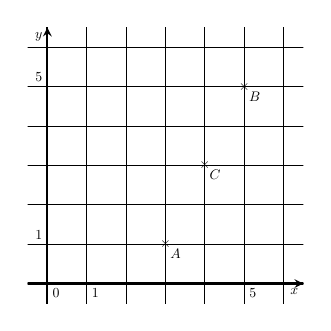
\begin{tikzpicture}[scale=0.5,every node/.style={scale=0.5}]
		%Points
		\clip (-0.5,-0.5) rectangle (6.5,6.5);
		\coordinate(O)at(0,0);
		\coordinate(I)at(1,0);
		\coordinate(J)at(0,1);
		\coordinate(xstart)at(-8,0);
		\coordinate(xend)at(8,0);
		\coordinate(ystart)at(0,-8);
		\coordinate(yend)at(0,8);
		\coordinate(A)at(3,1);
		\coordinate(B)at(5,5);
		\coordinate(C)at(4,3);
		\coordinate(D)at(4,-5);
		\coordinate(E)at(-7,4);
		\coordinate(F)at(-5,0);
		\coordinate(G)at(0,-3);
		\coordinate(H)at(0,7);
		%Étiquettes
	%	\draw (I) node[below right] {$1$};
	%	\draw (J) node[above left] {$1$};
		\draw [>=stealth,->] (O) -- (6.5,0) node[below left] {$x$};
		\draw [>=stealth,->] (O) -- (0,6.5) node[below left] {$y$};	
		%%%%%%%%%%%%%%%%%%%%%%%%%%%%%%%%%%%%
		%Axes
		\draw [thick] (xstart) -- (xend);
		\draw [thick] (ystart) -- (yend);
		%Flèches
	%	\draw [>=stealth,->] (O) -- (I);
	%	\draw [>=stealth,->] (O) -- (J);
		\draw [>=stealth,->] (O) -- (xend);
		\draw [>=stealth,->] (O) -- (yend);
		%Grille
		\draw [thin] (-8,-8)grid(8,8);
		%%%%%%%%%%%%%%%%%%%%%%%%%%%%%%%%%%%%
		%étiquettes
		\foreach \point in {A, ..., C}
			\draw(\point)node{$\times$};
		\foreach \point in {A, ..., C}
			\draw(\point)node[below right]{$\point$};	
		\foreach \r in {0, 1, 5}
	    	\draw[thick, below right] (\r,0) node{\r};
		\foreach \r in {1, 5}
	    	\draw[thick, above left] (0,\r) node{\r};
%		\only<9-|handout:2-3>{\draw[thick,red] (-0.5,-0.5) rectangle (6.5,6.5);}
	\end{tikzpicture}
	%}
	\end{center}
	\end{minipage}
	\begin{minipage}{0.2\textwidth}
		\begin{enumerate}[]
			\item $A(~~3~,~1~)$
			\item $B(~~5~,~5~)$
			\item $C(~~4~,~3~)$
%			\item<1->\only<1-4|handout:1>{$D(~~~~~,~~~~~)$}\only<5-9|handout:2>{$D(~4~,-5~)$}
%			\item<1->\only<1-5|handout:1>{$E(~~~~~,~~~~~)$}\only<6-9|handout:2>{$E(~-7~,~4~)$}
%			\item<1->\only<1-6|handout:1>{$F(~~~~~,~~~~~)$}\only<7-9|handout:2>{$F(~-5~,~0~)$}
%			\item<1->\only<1-7|handout:1>{$G(~~~~~,~~~~~)$}\only<8-9|handout:2>{$G(~0~,~-3~)$}
%			\item<1->\only<1-8|handout:1>{$H(~~~~~,~~~~~)$}\only<9-9|handout:2>{$H(~~0~,~7~)$}
		\end{enumerate}
	\end{minipage}
	\only<10-12|handout:2>{\begin{block}{Coordonnées}}
	\only<10-12|handout:2>{On repère un point dans le plan par ses \textbf{coordonnées}. Le point $A$ a pour coordonnées $(3,1)$. On appelle $3$ son \textbf{abscisse} et $1$ son \textbf{ordonnée}.}
	\only<10-12|handout:2>{\end{block}}
\end{frame}
%
%\subsection{Placer un point connaissant ses coordonnées}
%\begin{frame}
%\frametitle{Placer un point connaissant ses coordonnées}
%	\begin{minipage}{0.75\textwidth}
%	\begin{center}
%	%\fbox{
%	\begin{tikzpicture}[scale=0.5,every node/.style={scale=0.5}]
%		%Points
%		\coordinate(O)at(0,0);
%		\coordinate(I)at(1,0);
%		\coordinate(J)at(0,1);
%		\coordinate(xstart)at(-8,0);
%		\coordinate(xend)at(8,0);
%		\coordinate(ystart)at(0,-8);
%		\coordinate(yend)at(0,8);
%		\coordinate(A)at(5,3);
%		\coordinate(B)at(-2,3);
%		\coordinate(C)at(-2,-4);
%		\coordinate(D)at(6,2);
%		\coordinate(E)at(7,-4);
%		\coordinate(F)at(6,0);
%		\coordinate(G)at(0,3);
%		\coordinate(H)at(0,-7);
%		%Étiquettes
%%		\draw (I) node[below right] {$1$};
%%		\draw (J) node[above left] {$1$};
%		\draw (xend) node[below right] {$x$};
%		\draw (yend) node[above left] {$y$};	
%		%%%%%%%%%%%%%%%%%%%%%%%%%%%%%%%%%%%%
%		%Axes
%		\draw [thick] (xstart) -- (xend);
%		\draw [thick] (ystart) -- (yend);
%		%Flèches
%%		\draw [>=stealth,->] (O) -- (I);
%%		\draw [>=stealth,->] (O) -- (J);
%		\draw [>=stealth,->] (O) -- (xend);
%		\draw [>=stealth,->] (O) -- (yend);
%		%Grille
%		\draw [thin] (-8,-8)grid(8,8);
%		%%%%%%%%%%%%%%%%%%%%%%%%%%%%%%%%%%%%
%		%étiquettes
%		\only<2-|handout:2>{
%		\foreach \point in {A, ..., H}
%			\draw(\point)node{$\times$};
%		\foreach \point in {A, ..., H}
%			\draw(\point)node[below right]{$\point$};
%		}
%		\foreach \r in {0, 1, 5}
%	    	\draw[thick, below right] (\r,0) node{\r};
%		\foreach \r in {1, 5}
%	    	\draw[thick, above left] (0,\r) node{\r};  
%	\end{tikzpicture}
%	%}
%	\end{center}
%	\end{minipage}
%	\begin{minipage}{0.2\textwidth}
%		\begin{enumerate}[]
%			\item<1-|handout:1-> $A(~~5~,~3~)$
%			\item<1-|handout:1-> $B(~-2~,~3~)$
%			\item<1-|handout:1-> $C(-2,-4)$
%			\item<1-|handout:1-> $D(~~6~,~~2~)$
%			\item<1-|handout:1-> $E(~~7~,~-4)$
%			\item<1-|handout:1-> $F(~~6~,~~0~)$
%			\item<1-|handout:1-> $G(~~0~,~~3~)$
%			\item<1-|handout:1-> $H(~~0~,-7)$
%		\end{enumerate}
%	\end{minipage}
%\end{frame}
%

\section{Milieu d'un segment}
\subsection{Propriété admise}
\begin{frame}
\frametitle{3) Milieu d'un segment}
	\begin{center}
	\begin{tikzpicture}[scale=1,every node/.style={scale=1}]
		\coordinate (A) at (0,0);
		\coordinate (B) at (4,2);
		\draw (A) -- (B)	node[midway,above] {$M$}
							node[midway] {$\times$}
							node[near start,sloped] {$//$}
							node[near end,sloped] {$//$};
		\draw (A)			node[above] {$A$}
							node {$\times$};
		\draw (B)			node[above] {$B$}
							node {$\times$};
	\end{tikzpicture}
	\end{center}
	\begin{block}{Propriété}
	Soient $\pointcoord{A}{x_A}{y_A}$ et $\pointcoord{B}{x_B}{y_B}$ deux points du plan.\\ Soit $\pointcoord{M}{x_M}{y_M}$ milieu du segment $[AB]$.\\ Le point $M$ a pour coordonnées~:\\
	\[
	\pointcoord{M}{\dfrac{x_A+x_B}{2}}{\dfrac{y_A+y_B}{2}}
	\]

	\end{block}
\end{frame}

\begin{frame}
%\frametitle{2) Milieu d'un segment}
%	\begin{minipage}{0.75\textwidth}
%	\begin{center}
%	%\fbox{
%	\begin{tikzpicture}[scale=0.5,every node/.style={scale=0.5}]
%		%Points
%		\clip (-0.5,-0.5) rectangle (6.5,6.5);
%		\coordinate(O)at(0,0);
%		\coordinate(I)at(1,0);
%		\coordinate(J)at(0,1);
%		\coordinate(xstart)at(-8,0);
%		\coordinate(xend)at(8,0);
%		\coordinate(ystart)at(0,-8);
%		\coordinate(yend)at(0,8);
%		\coordinate(A)at(3,1);
%		\coordinate(B)at(5,5);
%		\coordinate(C)at(4,3);
%		\coordinate(D)at(4,-5);
%		\coordinate(E)at(-7,4);
%		\coordinate(F)at(-5,0);
%		\coordinate(G)at(0,-3);
%		\coordinate(H)at(0,7);
%		%Étiquettes
%	%	\draw (I) node[below right] {$1$};
%	%	\draw (J) node[above left] {$1$};
%		\draw [>=stealth,->] (O) -- (6.5,0) node[below left] {$x$};
%		\draw [>=stealth,->] (O) -- (0,6.5) node[below left] {$y$};	
%		%%%%%%%%%%%%%%%%%%%%%%%%%%%%%%%%%%%%
%		%Axes
%		\draw [thick] (xstart) -- (xend);
%		\draw [thick] (ystart) -- (yend);
%		%Flèches
%	%	\draw [>=stealth,->] (O) -- (I);
%	%	\draw [>=stealth,->] (O) -- (J);
%		\draw [>=stealth,->] (O) -- (xend);
%		\draw [>=stealth,->] (O) -- (yend);
%		%Grille
%		\draw [thin] (-8,-8)grid(8,8);
%		%%%%%%%%%%%%%%%%%%%%%%%%%%%%%%%%%%%%
%		%étiquettes
%		\foreach \point in {A, ..., C}
%			\draw(\point)node{$\times$};
%		\foreach \point in {A, ..., C}
%			\draw(\point)node[below right]{$\point$};	
%		\foreach \r in {0, 1, 5}
%	    	\draw[thick, below right] (\r,0) node{\r};
%		\foreach \r in {1, 5}
%	    	\draw[thick, above left] (0,\r) node{\r};
%%		\only<9-|handout:2-3>{\draw[thick,red] (-0.5,-0.5) rectangle (6.5,6.5);}
%	\end{tikzpicture}
%	%}
%	\end{center}
%	\end{minipage}
%	\begin{minipage}{0.2\textwidth}
%		\begin{enumerate}[]
%			\item $A(~~3~,~1~)$
%			\item $B(~~5~,~5~)$
%			\item $C(~~4~,~3~)$
%%			\item<1->\only<1-4|handout:1>{$D(~~~~~,~~~~~)$}\only<5-9|handout:2>{$D(~4~,-5~)$}
%%			\item<1->\only<1-5|handout:1>{$E(~~~~~,~~~~~)$}\only<6-9|handout:2>{$E(~-7~,~4~)$}
%%			\item<1->\only<1-6|handout:1>{$F(~~~~~,~~~~~)$}\only<7-9|handout:2>{$F(~-5~,~0~)$}
%%			\item<1->\only<1-7|handout:1>{$G(~~~~~,~~~~~)$}\only<8-9|handout:2>{$G(~0~,~-3~)$}
%%			\item<1->\only<1-8|handout:1>{$H(~~~~~,~~~~~)$}\only<9-9|handout:2>{$H(~~0~,~7~)$}
%		\end{enumerate}
%	\end{minipage}
	\begin{block}{Exemple}
	Soient $\pointcoord{A}{3}{1}$ et $\pointcoord{B}{5}{5}$ deux points du plan placés dans le repère $(O,I,J)$. Les coordonnées du point $C$ milieu de $[AB]$ sont~: \\
%	$\pointcoord{C}{\dfrac{3+5}{2}}{\dfrac{1+5}{2}}=$ 
%	$\pointcoord{C}{\dfrac{x_A+x_B}{2}}{\dfrac{y_A+y_B}{2}}$
	
	\[x_C = \dfrac{3+5}{2} = 4\]
	
	\[y_C = \dfrac{1+5}{2} = 3\]
	
	\[\text{Donc on a }\pointcoord{C}{4}{3}\]	
	\end{block}
\end{frame}


\begin{frame}
	\begin{block}{Exercice type n°1}
	Soient $\pointcoord{A}{10}{30}$ et $\pointcoord{M}{11}{18}$ deux points du plan placés dans le repère $(O,I,J)$.\\~\\ Déterminer les coordonnées du point~$B$ tel que $M$ soit le milieu du segment $[AB]$.\\
	\end{block}
\end{frame}

\begin{frame}
	\begin{block}{Exercice type n°2}
	Soient $\pointcoord{A}{8}{5}$, $\pointcoord{B}{20}{2}$, $\pointcoord{C}{22}{7}$ et $\pointcoord{D}{10}{10}$ quatre points du plan placés dans le repère $(O,I,J)$.\\~\\ Montrer que le quadrilatère $ABCD$ est un parallélogramme.
	\end{block}
\end{frame}

\begin{frame}
	\begin{block}{Exercice type n°3}
	Soient $\pointcoord{A}{2}{2}$, $\pointcoord{B}{20}{8}$, $\pointcoord{C}{26}{16}$ et $\pointcoord{D}{10}{8}$ quatre points du plan placés dans le repère $(O,I,J)$.\\~\\ Le quadrilatère $ABCD$ est-il un parallélogramme~?
	\end{block}
\end{frame}

\begin{frame}
	\begin{block}{Exercice type n°4}
	Soient $\pointcoord{A}{2}{2}$, $\pointcoord{B}{20}{8}$, $\pointcoord{C}{26}{16}$ trois points du plan placés dans le repère $(O,I,J)$.\\~\\ Déterminer les coordonnées du point $D$ pour que le quadrilatère $ABCD$ soit un parallélogramme.
	\end{block}
\end{frame}















%%%%%
%%%%%
%%%%%
%%%%%
%%%%%
%%%%%%\begin{frame}<0| handout:0>
%%%%%%
%%%%%%\begin{itemize}
%%%%%%  \item This one is always shown
%%%%%%  \item<1-> The first time (i.e. as soon as the slide loads)
%%%%%%  \item<2-> The second time
%%%%%%  \item<1-> Also the first time
%%%%%%  \only<1-1> {This one is shown at the first time, but it will hide soon (on the next event after the slide loads).}
%%%%%%\end{itemize}
%%%%%%
%%%%%%$$x=4$$
%%%%%%\pause
%%%%%%
%%%%%%$$x=4$$
%%%%%%\pause
%%%%%%
%%%%%%$$x=4$$
%%%%%%\pause
%%%%%%
%%%%%%$$x=4$$
%%%%%%\pause
%%%%%%
%%%%%%$$x=4$$
%%%%%%\end{frame}
%%%%%
%%%%%\section{Distance entre deux points}
%%%%%\subsection{Comment déterminer la distance entre deux points ?}
%%%%%\begin{frame}
%%%%%	\begin{center}
%%%%%	%\fbox{
%%%%%	\begin{tikzpicture}[scale=0.5,every node/.style={scale=0.5}]
%%%%%		%Points
%%%%%		\clip (-2,-2) rectangle (8,7);
%%%%%		\coordinate(O)at(0,0);
%%%%%		\coordinate(I)at(1,0);
%%%%%		\coordinate(J)at(0,1);
%%%%%		\coordinate(xstart)at(-2,0);
%%%%%		\coordinate(xend)at(7,0);
%%%%%		\coordinate(ystart)at(0,-2);
%%%%%		\coordinate(yend)at(0,6);
%%%%%		\coordinate(V)at(-1,-1);
%%%%%		\coordinate(B)at(2,-1);
%%%%%		\coordinate(R)at(2,3);
%%%%%		\coordinate(A)at(6,-1);
%%%%%		%Étiquettes
%%%%%	%	\draw (I) node[below right] {$1$};
%%%%%	%	\draw (J) node[above left] {$1$};
%%%%%		\only<4-|handout:3->{\draw (xend) node[below right] {$x$};}
%%%%%		\only<4-|handout:3->{\draw (yend) node[above left] {$y$};}
%%%%%		%%%%%%%%%%%%%%%%%%%%%%%%%%%%%%%%%%%%
%%%%%		%Axes
%%%%%		\only<3-|handout:3->{\draw [thick] (xstart) -- (xend);}
%%%%%		\only<3-|handout:3->{\draw [thick] (ystart) -- (yend);}
%%%%%		%Flèches
%%%%%	%	\draw [>=stealth,->] (O) -- (I);
%%%%%	%	\draw [>=stealth,->] (O) -- (J);
%%%%%		\only<3-|handout:3->{\draw [>=stealth,->] (O) -- (xend);}
%%%%%		\only<3-|handout:3->{\draw [>=stealth,->] (O) -- (yend);}
%%%%%		%Grille
%%%%%		\only<3-|handout:3->{\draw [thin] (-2,-2)grid(7,6);}
%%%%%		%%%%%%%%%%%%%%%%%%%%%%%%%%%%%%%%%%%%
%%%%%		%étiquettes
%%%%%		\foreach \point in {V,B,R,A}
%%%%%			\draw(\point)node{$\times$};
%%%%%		\foreach \point in {V,B,R,A}
%%%%%			\draw(\point)node[below right]{$\point$};	
%%%%%		\only<3-|handout:3->{
%%%%%    	\draw[thick, below right] (0,0) node{0};
%%%%%    	\draw[thick, below right] (1,0) node{20};
%%%%%    	\draw[thick, below right] (5,0) node{100};
%%%%%    	\draw[thick, above left] (0,1) node{20};
%%%%%    	\draw[thick, above left] (0,5) node{100};
%%%%%	    }
%%%%%		\only<1-|handout:1->{\draw [thick,dashed,red] (V) -- (A);}
%%%%%		\only<1-|handout:1->{\draw [thick,dashed,red] (B) -- (R);}
%%%%%		
%%%%%		\only<6-|handout:5->{\draw [thick,red] (B) -- (R) node[midway,above,sloped] {$80$};}
%%%%%		\only<7-|handout:6->{\draw [thick,green] (V) -- (R) node[midway,above,sloped] {$100$};}
%%%%%		\only<4-4|handout:4-4>{\draw [thick,blue] (V) -- (5,-1) node[near end,below,sloped] {$120$};}
%%%%%		\only<4-6|handout:4-5>{\draw [thick,blue] (V) -- (R) node[midway,above,sloped] {$?$};}
%%%%%		\only<5-|handout:5->{\draw [thick,red] (V) -- (B) node[midway,below,sloped] {$60$};}
%%%%%		
%%%%%	\end{tikzpicture}
%%%%%	%}
%%%%%	\\[2em]	
%%%%%	À quelques kilomètres de l'arrivée d'une course automobile, le véhicule situé en $V$ doit prendre une décision~:\\	
%%%%%	Peut-il tenter d'aller jusqu'à l'arrivée~$A$ directement ou bien doit-il passer par le ravitaillement~$R$~? Vous devez l'aider à prendre cette décision. Que lui conseillez-vous ?\\ \only<2-|handout:2->{\textcolor{red}{Il lui reste 120km d'autonomie.}}~\\ \only<7-|handout:6>{\textcolor{green}{Pythagore : VR $= 100$}}
%%%%%	\end{center}
%%%%%\end{frame}
%%%%%\begin{frame}
%%%%%	\begin{block}{Propriété}
%%%%%	Soit $\pointcoord{A}{x_A}{y_A}$ et $\pointcoord{B}{x_B}{y_B}$ dans un repère \textbf{orthonormé}. La distance $AB$ est égale à~: $$AB=\sqrt{\left(x_B-x_A\right)^2+\left(y_B-y_A\right)^2}$$
%%%%%	
%%%%%	\end{block}
%%%%%\end{frame}
%%%%%
%%%%%\begin{frame}
%%%%%	\begin{alertblock}{Démonstration}
%%%%%	On considère le point $\pointcoord{C}{x_B}{y_A}$.\\\pause
%%%%%	On suppose que $x_B \neq x_A$ ET $y_B \neq y_A$.\\\pause
%%%%%	Les axes du repère sont perpendiculaires donc le triangle $ABC$ est rectangle en $C$.\\\pause
%%%%%	Par le théorème de Pythagore, $AB^2=AC^2+BC^2$.\\\pause
%%%%%	Or $AC=x_B-x_A$ ou $AC=x_A-x_B$. Dans les deux cas $AC^2=\left(x_B-x_A\right)^2$.\pause ~ De même, $BC^2=\left(y_B-y_A\right)^2$.\\\pause
%%%%%	Les unités étant les mêmes sur les deux axes, on a alors~: $AB^2=\left(x_B-x_A\right)^2+\left(y_B-y_A\right)^2$\\\pause
%%%%%	d'où \fbox{$AB=\sqrt{\left(x_B-x_A\right)^2+\left(y_B-y_A\right)^2}$}\\\pause
%%%%%	On vérifie que la formule reste vraie si $x_B=x_A$ ou $y_B=y_A$.
%%%%%	\end{alertblock}
%%%%%\end{frame}
%%%%%
%%%%%
%%%%%
%%%%%
%%%%%
%%%%%
%%%%%
%%%%%
%%%%%
%%%%%
%%%%%
%%%%%
%%%%%
%%%%%
%%%%%
%%%%%
%%%%%
%%%%%
%%%%%
%%%%%%\begin{frame}
%%%%%%  \begin{alertblock}{toto}
%%%%%%  titi
%%%%%%  \end{alertblock}
%%%%%%  \begin{block}{toto}
%%%%%%  titi
%%%%%%  \end{block}
%%%%%%  \begin{exampleblock}{toto}
%%%%%%  titi
%%%%%%  \end{exampleblock}
%%%%%%
%%%%%%  \begin{enumerate}
%%%%%%    \item General Libraries
%%%%%%      \begin{itemize}
%%%%%%        \item LibBaseGeneralClasses
%%%%%%        \item LibGeneralClasses
%%%%%%      \end{itemize}
%%%%%%    \visible<2->{
%%%%%%    \item Code
%%%%%%    \begin{itemize}
%%%%%%      \item LibBaseEFIT3DClasses
%%%%%%      \item LibEFIT3DBoundaryConditions
%%%%%%      \item LibEFIT3DClasses
%%%%%%      \item LibEFIT3DFactories
%%%%%%    \end{itemize}
%%%%%%    }
%%%%%%  \end{enumerate}
%%%%%%\end{frame}
%%%%%%\subsection{Placer un point connaissant ses coordonnées}
%%%%%%\begin{frame}
%%%%%%  \begin{enumerate}
%%%%%%    \item<1-| alert@1> Create dictionaries from sources -- specific to ROOT
%%%%%%    \visible<2-> {\item<2-| alert@2> Create libraries from sources + dictionaries}
%%%%%%    \visible<3-> {\item<3-| alert@3> Compile the main program with created libraries}
%%%%%%  \end{enumerate}
%%%%%%    \begin{center}
%%%%%%      %\includegraphics[width=0.6\textwidth]{./../pictures/makefile.eps}
%%%%%%    \end{center}
%%%%%%\end{frame}
%%%%%%
%%%%%%\subsection{Issues due to code extraction}
%%%%%%\begin{frame}
%%%%%%\begin{itemize}
%%%%%%  \item<1-| alert@1> Errors
%%%%%%  \begin{itemize}
%%%%%%      \item<1-| alert@1> Calls to unused functions
%%%%%%      \item<1-| alert@1> Broken test functions
%%%%%%  \end{itemize}
%%%%%%  \visible<2-> {
%%%%%%    \item<2-| alert@2> Warnings
%%%%%%    \begin{itemize}
%%%%%%      \item<2-| alert@2> Unused variables
%%%%%%      \item<2-| alert@2> Undefined variables
%%%%%%    \end{itemize}
%%%%%%  }
%%%%%%\end{itemize}
%%%%%%\end{frame}
%%%%%
%%%%%
%%%%%%\section{Simulations}
%%%%%%\subsection{Accuracy}
%%%%%%
%%%%%%\begin{frame}
%%%%%%\frametitle{Checking the code}
%%%%%%\begin{figure}[h!]
%%%%%%	\centering
%%%%%%	%\includegraphics[width=0.7\textwidth]{./../pictures/0.5MHZ-BW1.eps}
%%%%%%	\caption[0.50~MHz, Bandwidth~1.0]{Same configuration files, looking for the same outcome}
%%%%%%	\label{fig:0.5-1.0_first}
%%%%%%\end{figure}
%%%%%%\end{frame}
%%%%%%
%%%%%%
%%%%%%\subsection{Bandwidth}
%%%%%%
%%%%%%\begin{frame}
%%%%%%\frametitle{Center frequency = 1.88~MHz}
%%%%%%\only<1>{
%%%%%%\begin{figure}[h!]
%%%%%%	\centering
%%%%%%	%\includegraphics[width=0.7\textwidth]{./../pictures/1.88MHZ-BW1.eps}
%%%%%%	\caption[1.88~MHz, Bandwidth~1.0]{Bandwidth parameter = 1.0. On this picture we can see a wave propagating from the transducer (bottom) through the material towards the top of the piece.}
%%%%%%	\label{fig:1.88-1.0}
%%%%%%\end{figure}
%%%%%%}
%%%%%%
%%%%%%\only<2>{
%%%%%%\begin{figure}[h!]
%%%%%%	\centering
%%%%%%	%\includegraphics[width=0.7\textwidth]{./../pictures/1.88MHZ-BW2.eps}
%%%%%%	\caption[1.88~MHz, Bandwidth~2.0]{Bandwidth parameter = 2.0}
%%%%%%	\label{fig:1.88-2.0}
%%%%%%\end{figure}
%%%%%%}
%%%%%%
%%%%%%\only<3>{
%%%%%%\begin{figure}[h!]
%%%%%%	\centering
%%%%%%	%\includegraphics[width=0.7\textwidth]{./../pictures/1.88MHZ-BW3.eps}
%%%%%%	\caption[1.88~MHz, Bandwidth~3.0]{Bandwidth parameter = 3.0}
%%%%%%	\label{fig:1.88-3.0}
%%%%%%\end{figure}
%%%%%%}
%%%%%%
%%%%%%
%%%%%%\only<4>{
%%%%%%\begin{figure}[h!]
%%%%%%	\centering
%%%%%%	%\includegraphics[width=0.7\textwidth]{./../pictures/1.88MHZ-BW6.eps}
%%%%%%	\caption[1.88~MHz, Bandwidth~6.0]{Bandwidth parameter = 6.0}
%%%%%%	\label{fig:1.88-6.0}
%%%%%%\end{figure}
%%%%%%}
%%%%%%
%%%%%%\only<5>{
%%%%%%\begin{figure}[h!]
%%%%%%	\centering
%%%%%%	%\includegraphics[width=0.7\textwidth]{./../pictures/1.88MHZ-BW10.eps}
%%%%%%	\caption[1.88~MHz, Bandwidth~10.0]{Bandwidth parameter = 10.0}
%%%%%%	\label{fig:1.88-10.0}
%%%%%%\end{figure}
%%%%%%}
%%%%%%\end{frame}
%%%%%
%%%%%
%%%%%%\begin{frame}
%%%%%%The right bandwidth parameter is between 6.0 and 10.0. If I had had more time at the end of my internship I would have run more simulations to determine it but the simulation with a 1.88~MHz center frequency is very time consuming (almost one day according to Figure~\ref{fig:time}).
%%%%%%
%%%%%%We will make some simulations in subsection~\ref{sec:freq} and for each frequency we will also change the bandwidth parameter.
%%%%%%first:
%%%%%%\begin{center}
%%%%%%$$Bandwidth parameter = 1.0$$
%%%%%%and then:
%%%%%%$$Bandwidth parameter = 2.0$$
%%%%%%\end{center}
%%%%%%
%%%%%%\end{frame}
%%%%%
%%%%%%\subsection{Frequency}
%%%%%%\label{sec:freq}
%%%%%%\begin{frame}
%%%%%%\frametitle{Center frequency = 0.5~MHz}
%%%%%%
%%%%%%\begin{figure}[H]
%%%%%%\begin{minipage}[t]{0.45\textwidth}
%%%%%%	\centering
%%%%%%	%%\includegraphics[width=\textwidth]{./../pictures/0.5MHZ-BW1.eps}
%%%%%%	\caption[0.50~MHz, Bandwidth~1.0]{Bandwidth = 1.0}
%%%%%%	\label{fig:0.5-1.0}
%%%%%%\end{minipage}\hfill
%%%%%%\begin{minipage}[t]{0.45\textwidth}
%%%%%%	\centering
%%%%%%	%\includegraphics[width=\textwidth]{./../pictures/0.5MHZ-BW2.eps}
%%%%%%	\caption[0.50~MHz, Bandwidth~2.0]{Bandwidth = 2.0}
%%%%%%	\label{fig:0.5-2.0}
%%%%%%\end{minipage}
%%%%%%\end{figure}
%%%%%%
%%%%%%
%%%%%%In this case, we can see the bandwidth parameter actually acts on the signal. The chosen center frequency allows to make simulations fast but we can't really see what happens.
%%%%%%\end{frame}
%%%%%%
%%%%%%\begin{frame}
%%%%%%\frametitle{Center frequency = 0.94~MHz}
%%%%%%
%%%%%%\begin{figure}[H]
%%%%%%\begin{minipage}[t]{0.45\textwidth}
%%%%%%	\centering
%%%%%%	%\includegraphics[width=\textwidth]{./../pictures/0.94MHZ-BW1.eps}
%%%%%%	\caption[0.94~MHz, Bandwidth~1.0]{Bandwidth = 1.0}
%%%%%%	\label{fig:0.94-1.0}
%%%%%%\end{minipage}\hfill
%%%%%%\begin{minipage}[t]{0.45\textwidth}
%%%%%%	\centering
%%%%%%	%\includegraphics[width=\textwidth]{./../pictures/0.94MHZ-BW2.eps}
%%%%%%	\caption[0.94~MHz, Bandwidth~2.0]{Bandwidth = 2.0}
%%%%%%	\label{fig:0.94-2.0}
%%%%%%\end{minipage}
%%%%%%\end{figure}
%%%%%%\end{frame}
%%%%%%
%%%%%%
%%%%%%\begin{frame}
%%%%%%\frametitle{Center frequency = 1.0~MHz}
%%%%%%
%%%%%%\begin{figure}[H]
%%%%%%\begin{minipage}[t]{0.45\textwidth}
%%%%%%	\centering
%%%%%%	%\includegraphics[width=\textwidth]{./../pictures/1.0MHZ-BW1.eps}
%%%%%%	\caption[1.0~MHz, Bandwidth~1.0]{Bandwidth = 1.0}
%%%%%%	\label{fig:1.0-1.0}
%%%%%%\end{minipage}\hfill
%%%%%%\begin{minipage}[t]{0.45\textwidth}
%%%%%%	\centering
%%%%%%	%\includegraphics[width=\textwidth]{./../pictures/1.0MHZ-BW2.eps}
%%%%%%	\caption[1.0~MHz, Bandwidth~2.0]{Bandwidth = 2.0}
%%%%%%	\label{fig:1.0-2.0}
%%%%%%\end{minipage}
%%%%%%\end{figure}
%%%%%%\end{frame}
%%%%%%
%%%%%%
%%%%%%\begin{frame}
%%%%%%For 0.5, 0.94 and 1.0~MHz, the wave and its reflection are completely overlapping. This is bad to detect defects or flaws especially if they are small.
%%%%%%\end{frame}
%%%%%%
%%%%%%\begin{frame}
%%%%%%\frametitle{Center frequency = 1.5~MHz}
%%%%%%
%%%%%%\begin{figure}[H]
%%%%%%\begin{minipage}[t]{0.45\textwidth}
%%%%%%	\centering
%%%%%%	%\includegraphics[width=\textwidth]{./../pictures/1.5MHZ-BW1.eps}
%%%%%%	\caption[1.5~MHz, Bandwidth~1.0]{Bandwidth = 1.0}
%%%%%%	\label{fig:1.5-1.0}
%%%%%%\end{minipage}\hfill
%%%%%%\begin{minipage}[t]{0.45\textwidth}
%%%%%%	\centering
%%%%%%	%\includegraphics[width=\textwidth]{./../pictures/1.5MHZ-BW2.eps}
%%%%%%	\caption[1.5~MHz, Bandwidth~2.0]{Bandwidth = 2.0}
%%%%%%	\label{fig:1.5-2.0}
%%%%%%\end{minipage}
%%%%%%\end{figure}
%%%%%%\end{frame}
%%%%%
%%%%%%\begin{frame}
%%%%%%\frametitle{Center Frequency = 1.88~MHz}
%%%%%%
%%%%%%\begin{figure}[H]
%%%%%%\begin{minipage}[t]{0.45\textwidth}
%%%%%%	\centering
%%%%%%	%\includegraphics[width=\textwidth]{./../pictures/1.88MHZ-BW1.eps}
%%%%%%	\caption[1.88~MHz, Bandwidth~1.0]{Bandwidth = 1.0}
%%%%%%	\label{fig:1.88-1.0}
%%%%%%\end{minipage}\hfill
%%%%%%\begin{minipage}[t]{0.45\textwidth}
%%%%%%	\centering
%%%%%%	%\includegraphics[width=\textwidth]{./../pictures/1.88MHZ-BW2.eps}
%%%%%%	\caption[1.88~MHz, Bandwidth~2.0]{Bandwidth = 2.0}
%%%%%%	\label{fig:1.88-2.0}
%%%%%%\end{minipage}
%%%%%%\end{figure}
%%%%%%\end{frame}
%%%%%
%%%%%
%%%%%%\begin{frame}
%%%%%%\frametitle{Center frequency = 2.0~MHz}
%%%%%%
%%%%%%\begin{figure}[H]
%%%%%%\begin{minipage}[t]{0.45\textwidth}
%%%%%%	\centering
%%%%%%	%\includegraphics[width=\textwidth]{./../pictures/2.0MHZ-BW1.eps}
%%%%%%	\caption[2.0~MHz, Bandwidth~1.0]{Bandwidth = 1.0}
%%%%%%	\label{fig:2.0-1.0}
%%%%%%\end{minipage}\hfill
%%%%%%\begin{minipage}[t]{0.45\textwidth}
%%%%%%	\centering
%%%%%%	%\includegraphics[width=\textwidth]{./../pictures/2.0MHZ-BW2.eps}
%%%%%%	\caption[2.0~MHz, Bandwidth~2.0]{Bandwidth = 2.0}
%%%%%%	\label{fig:2.0-2.0}
%%%%%%\end{minipage}
%%%%%%\end{figure}
%%%%%%\end{frame}
%%%%%%
%%%%%%
%%%%%%\begin{frame}
%%%%%%\frametitle{Center frequency = 2.5~MHz}
%%%%%%
%%%%%%The code can't allocate enough memory.
%%%%%%
%%%%%%\end{frame}
%%%%%%
%%%%%%
%%%%%%\begin{frame}
%%%%%%\frametitle{Execution time}
%%%%%%
%%%%%%\begin{figure}[h!]
%%%%%%	\centering
%%%%%%	%\includegraphics[width=0.7\textwidth]{./../files/time.eps}
%%%%%%	\caption[Execution time of the EFIT code]{Execution time of the EFIT code}
%%%%%%	\label{fig:time}
%%%%%%\end{figure}
%%%%%%\end{frame}
%%%%%%
%%%%%%
%%%%%%\begin{frame}
%%%%%%\frametitle{Memory usage}
%%%%%%
%%%%%%\begin{figure}[h!]
%%%%%%	\centering
%%%%%%	%\includegraphics[width=0.7\textwidth]{./../files/memory.eps}
%%%%%%	\caption[Memory usage of the EFIT code]{Memory usage of the EFIT code}
%%%%%%	\label{fig:memory}
%%%%%%\end{figure}
%%%%%%\end{frame}
%%%%%%
%%%%%%\subsection{Squared area}
%%%%%%\begin{frame}
%%%%%%\begin{itemize}
%%%%%%  \item<1-| alert@1> Unexpected wave
%%%%%%  \item<2-| alert@2> Reflection
%%%%%%  \item<3-| alert@3> Dimensions
%%%%%%\end{itemize}
%%%%%%\end{frame}
%%%%%%
%%%%%%\begin{frame}
%%%%%%\begin{itemize}
%%%%%%  \item<1-| alert@1> Squared $3.75~cm$ piece
%%%%%%  \item<2-| alert@2> Squared $4.75~cm$ piece and bigger
%%%%%%\end{itemize}
%%%%%%\end{frame}
%%%%%
%%%%%
%%%%%%\section{Documentation}
%%%%%%\subsection*{Introduction}
%%%%%%\begin{frame}
%%%%%%\begin{itemize}
%%%%%%  \item<1-| alert@1> Rolf Scheben
%%%%%%  \visible<2-> {\item<2-| alert@2> C++ / ROOT Framework}
%%%%%%  \visible<3-> {\item<3-| alert@3> How to use it from scratch}
%%%%%%  \visible<4-> {\item<4-| alert@4> Install Framework}
%%%%%%  \visible<5-> {\item<5-| alert@5> Compile code}
%%%%%%  \visible<6-> {\item<6-| alert@6> Configuration file}
%%%%%%  \visible<7-> {\item<7-| alert@7> Run code}
%%%%%%\end{itemize} 
%%%%%%\end{frame}
%%%%%%
%%%%%%
%%%%%%
%%%%%%\subsection*{Install the Framework}
%%%%%%
%%%%%%\begin{frame}
%%%%%%\frametitle{ROOT Framework v5.28}
%%%%%%
%%%%%%\begin{itemize}
%%%%%%  \item Compatibility
%%%%%%  \item Same version
%%%%%%  \item Even if new versions
%%%%%%\end{itemize}
%%%%%%\end{frame}
%%%%%%
%%%%%%
%%%%%%\begin{frame}
%%%%%%\frametitle{ROOT Framework v5.28}
%%%%%%
%%%%%%\begin{itemize}
%%%%%%\item Extract
%%%%%%\item Configure
%%%%%%\item Compile
%%%%%%\item Enable
%%%%%%\end{itemize}
%%%%%%\end{frame}
%%%%%%
%%%%%%
%%%%%%
%%%%%%\subsection*{Compile the code}
%%%%%%\begin{frame}
%%%%%%\frametitle{Makefile.csh}
%%%%%%
%%%%%%set HOME = /path/to/your/home
%%%%%%
%%%%%%set BaseDirectory = \${HOME}/EFIT
%%%%%%\end{frame}
%%%%%%
%%%%%%\subsection*{What does this script do?}
%%%%%%
%%%%%%\subsection*{The configuration files}
%%%%%%\begin{frame}
%%%%%%Configuration\_Standard.sim
%%%%%%
%%%%%%Configuration.sim
%%%%%%\end{frame}
%%%%%%
%%%%%%\begin{frame}
%%%%%%\frametitle{Modules}
%%%%%%Among the available modules in the code and for our needs we will use these modules:
%%%%%%
%%%%%%\begin{itemize}
%%%%%%  \item UseModule Simulation
%%%%%%  \item UseModule:Simulation AScan
%%%%%%\end{itemize}
%%%%%%
%%%%%%\end{frame}
%%%%%%
%%%%%%
%%%%%%
%%%%%%\begin{frame}
%%%%%%\frametitle{Transmitter}
%%%%%%
%%%%%%\begin{itemize}
%%%%%%\visible<1->{
%%%%%%  \item<1-| alert@1> Transmitter:Load                                   true
%%%%%%}
%%%%%%\visible<2->{
%%%%%%  \item<2-| alert@2> Transmitter:OrientationPhi                         0
%%%%%%  \item<2-| alert@2> Transmitter:OrientationTheta                       0
%%%%%%  \item<2-| alert@2> Transmitter:OrientationAlpha                       0
%%%%%%}
%%%%%%\visible<3->{
%%%%%%  \item<3-| alert@3> Transmitter:CenterPointX                           0
%%%%%%  \item<3-| alert@3> Transmitter:CenterPointY                           0
%%%%%%  \item<3-| alert@3> Transmitter:CenterPointZ                          -0.038
%%%%%%}
%%%%%%\end{itemize}
%%%%%%\end{frame}
%%%%%%
%%%%%%
%%%%%%\begin{frame}
%%%%%%\frametitle{Transmitter geometry}
%%%%%%
%%%%%%Transmitter:Geometry Circular Ellipsoid Rectangular
%%%%%%\vspace{1cm}
%%%%%%
%%%%%%\textbf{Circular}
%%%%%%\begin{itemize}
%%%%%%\item Transmitter:Circular:Radius
%%%%%%\end{itemize}
%%%%%%
%%%%%%\visible<2->{
%%%%%%\textbf{Ellipsoid}
%%%%%%\begin{itemize}
%%%%%%\item Transmitter:Ellipsoid:HalfAxisX
%%%%%%\item Transmitter:Ellipsoid:HalfAxisY
%%%%%%\end{itemize}
%%%%%%}
%%%%%%
%%%%%%\visible<3->{
%%%%%%\textbf{Rectangular}
%%%%%%\begin{itemize}
%%%%%%\item Transmitter:Rectangular:LengthX
%%%%%%\item Transmitter:Rectangular:LengthY
%%%%%%\end{itemize}
%%%%%%}
%%%%%%\end{frame}
%%%%%%
%%%%%%
%%%%%%
%%%%%%\begin{frame}
%%%%%%\frametitle{Amplitude - Frequency - Bandwidth}
%%%%%%Transmitter:Signal:Formula:ParameterValues         1e-12,1.0e6,1.0
%%%%%%
%%%%%%\vspace{1cm}The Bandwidth parameter influences the pulse length. The bigger the Bandwidth parameter, the shorter the pulse length.
%%%%%%\end{frame}
%%%%%%
%%%%%%
%%%%%%
%%%%%%\begin{frame}
%%%%%%\frametitle{Geometry dimensions}
%%%%%%\vfill
%%%%%%GeneralGeometryGenerator:GeometrySource                      HardCoded
%%%%%%\vfill
%%%%%%GeneralGeometryGenerator:HardCodedGeometry:OffsetX           0
%%%%%%\vfill
%%%%%%GeneralGeometryGenerator:HardCodedGeometry:OffsetY           0
%%%%%%\vfill
%%%%%%GeneralGeometryGenerator:HardCodedGeometry:OffsetZ           0
%%%%%%\vfill
%%%%%%GeneralGeometryGenerator:HardCodedGeometry:LengthX           0.03
%%%%%%\vfill
%%%%%%GeneralGeometryGenerator:HardCodedGeometry:LengthY           0.03
%%%%%%\vfill
%%%%%%GeneralGeometryGenerator:HardCodedGeometry:LengthZ           0.03
%%%%%%\vfill
%%%%%%\end{frame}
%%%%%%
%%%%%%
%%%%%%\subsection*{Use the code}
%%%%%%\begin{frame}
%%%%%%\frametitle{Issues}
%%%%%%
%%%%%%\begin{itemize}
%%%%%%  \item Memory
%%%%%%  \item Disk space
%%%%%%\end{itemize}
%%%%%%\end{frame}	
%%%%%%
%%%%%%
%%%%%%\subsection*{Extract the data}
%%%%%%\begin{frame}
%%%%%%\frametitle{Extract the results}
%%%%%%
%%%%%%Use the two .C files to draw pictures.
%%%%%%\begin{itemize}
%%%%%%  \vspace{0.5cm}
%%%%%%  \item Write\ldots.C : to choose the timestep
%%%%%%  \vspace{0.5cm}
%%%%%%  \item Read\ldots.C : to choose which cuts to draw
%%%%%%  \vspace{0.5cm}
%%%%%%
%%%%%%    if ( CounterX == (int)(NrXBins/2) )
%%%%%%		
%%%%%%    if ( CounterY == (int)(NrYBins/2) )
%%%%%%		
%%%%%%    if ( CounterZ == (int)(NrZBins/2) )
%%%%%%\end{itemize}
%%%%%%
%%%%%%\end{frame}
%%%%%
%%%%%
%%%%%%\section{Conclusion}
%%%%%%\subsection*{Improvements}
%%%%%%\begin{frame}
%%%%%%\begin{itemize}
%%%%%%  \item Anisotropic
%%%%%%  \item Flaws
%%%%%%  \item Parallel
%%%%%%\end{itemize}
%%%%%%\end{frame}

\end{document}
